\chapter{O problema da latência}
\label{ch:2}

\section{Por que a latência importa ?}
A principal motivação do projeto RAMCloud é criar um sistema de armazenamento de dados com uma latência
consideravelmente menor do que os outros sistemas existentes. Tipicamente, aplicações web de larga escala
são executadas em muitos servidores dentro de um \emph{datacenter}, o qual possui máquinas separadas para
executar o código da aplicação e armazenar os dados~\ref{fig:i1}. Quando essa aplicação recebe uma requisição, é necessário
acessar dados que estão no servidor de dados, o que leva de 0.5ms a 10ms. 
\par
Devido à latência de acesso aos dados, uma aplicação que atenda milhões ou até mesmo bilhões de usuários 
não consegue processar muitas requisiçoes de dados aleatórios para uma dada requisição do usuário. Por exemplo, 
para que o Facebook possa ter um tempo de resposta rasoável só é possível que ele faça cerca de 150 requisições
de dados por requisição de usuário (ainda assim utilizando servidores de cache), o que acaba por limitar suas
funcionalidades.   
\par

O propósito do projeto RAMCloud é conseguir prover a menor latência possível para pequenos acessos aleatórios em 
aplicações web de larga escala. Com uma latência de acesso de cerca de 5$\mu$s é uma melhora de 50 a 1000x sobre
os sistemas de armazenamento de dados atuais.


%\begin{figure}[H]
%\begin{minted}[frame=single,linenos,mathescape]{html}
%<!DOCTYPE html>
%<html>
%    <head>
%        <meta charset="UTF-8">
%        <title>Titulo do documento</title>
%    </head>
%    <body>
%        <!-- Conteudo do documento -->
%    </body>
%</html>
%\end{minted}
%\caption{Estrutura básica de um documento HTML}
%\label{lst:html}
%\end{figure}

\begin{figure}[H]\centering
  \centerline{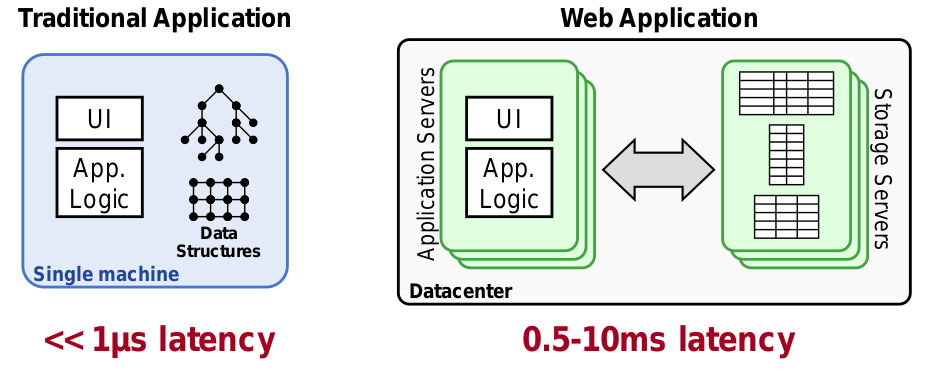
\includegraphics[width=\textwidth]{figuras/i1.png}}
  \caption{Em uma aplicaçao tradicional, os dados e o código estão na mesma máquina (latência de 50-100ns). Já em uma aplicação web escalável, como
  os dados e o código da aplicação estão em máquinas separadas, a latência pode chegar a até 10ms.}\label{fig:i1}
\end{figure}

\section{Atingindo baixa latência}

O principal obstaculo para atingir latências da ordem de 5$\mu$s a 10$\mu$s é a infraestrutura de rede. No início do projeto, no ano de 2009, o tempo típico de uma RPC\footnote{RPC - Remote Procedure Call ou Chamada de procedimento remoto é, basicamente, a operação que permite que um processo possa se comunicar ou outro processo em outra máquina geralmente por meio da rede} era de centenas de $\mu$s~\ref{fig:i2}. Além disso, os prórpios mecanismos do sistema operacional contribuem para aumentar a latência como chamadas ao kernel, a pilha de rede, interrupções, mecanismos de sincronização e o tempo de comunicação entre a CPU e a placa de rede.

\begin{figure}[H]\centering
  \centerline{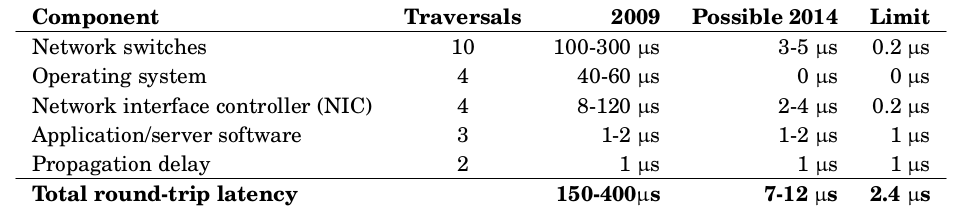
\includegraphics[width=\textwidth]{figuras/i2.png}}
  \caption{Latência média por componente uma uma RPC. \emph{Traversals}: quantas vezes um pacote precisa passar por cada componente em uma 
  requisição completa (round-trip). \emph{2009}: latência típica de um datacenter em 2009. \emph{Possible 2014}: latência possível de se atingir
  em 2014 a um custo razoável.}\label{fig:i2}
\end{figure}

\par

Mesmo com os avanços da tecnologia, a maior parte da latência ainda é gasta na rede ou na placa de rede, o que deixa cerca de 1$\mu$s para o sistema processar cada RPC. Sendo assim, para atingir esse objetivo foi preciso desenvolver um sistema no qual: 
\begin{itemize}
\item Servidores e aplicações precisam enviar e receber pacotes sem passar pelo kernel do sistema operacional;
\item Mecanismos de sincronização precisam ser evitados;
\item Minimizar os erros de coerência de cache;
\item Elimizar os mecanismos de \emph{batching} da placa de rede, onde um certo número de pacotes é acumulado e transmitidos de uma só vez.
\end{itemize}

No RAMCloud os registradores da placa de rede são mapeados diretamente no espaço de memória da aplicação, permitindo uma comunicação direta entre aplicaçao e placa de rede. Além disso, se uma \emph{thread} está esperando pela resposta de uma RPC, ao invés de ir dormir, ela fica constanstemente verificando a placa de rede. Essa técnica, chamada de \emph{busy waiting} (espera ocupada em português), ajuda a minimizar a latência da troca de contexto do sistema operacional.
\par 
Embora a melhor maneira de se minimizar a latência seja utilizar uma única thread para tratar todas as requisições, para garantir a tolerância a falhas os servidores RAMCloud utilizam múltiplas threads: uma única \emph{dispatch thread} e várias \emph{worker threads}. A \emph{dispatch thread} trata de toda a comunicação de rede (requisições e respostas) e também tem a função de selecionar uma \emph{worker thread} para processar cada requisição. Essa comunicação entre threads também é realizada pela técnica de busy waiting. 
